\chapter{Evaluation}
\label{chap:evaluation}

This chapter evaluates the project as a whole focusing on the development process, and whether the project meets the requirements set out in \autorefp{chap:requirements}. The chapter will also discuss the limitations of the project and potential future work.

\section{Project Timeline and Management}
\label{evaluation:timeline-management}

During the early stages of the academic year, starting a project was exciting and was progressing well. The problem proved challenging over time, yet rewarding when understanding the fundamentals that build route planning systems. Time management, planning and determining theoretical deadlines for development and report writing were crucial to ensuring steady progression despite the pressing deadlines of other modules. Due to this, the project swiftly began to move ahead of schedule, resulting in the initial Gantt chart \see{fig:initial-gantt} being revised to adjust for the rapid progress \see{fig:final-gantt}.

\newpage
\begin{landscape}
\begin{figure}[ht!]
    \centering
    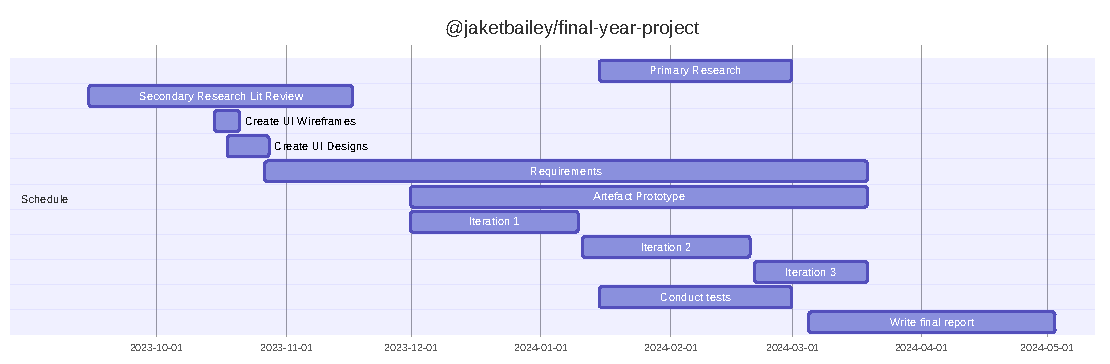
\includegraphics[width=1\linewidth]{figures/Old FYP Gantt - Timeline 1.pdf}
    \caption{Initial Gantt Chart}
    \label{fig:initial-gantt}
\end{figure}

\begin{figure}[h!]
    \centering
    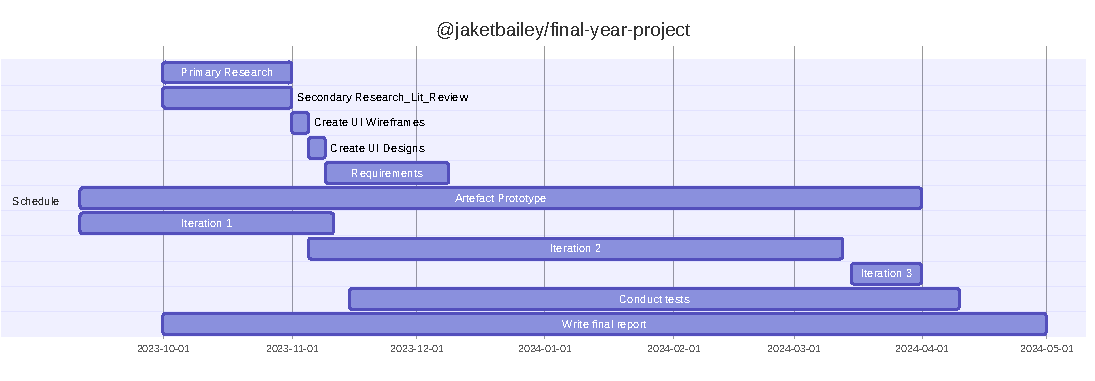
\includegraphics[width=1\linewidth]{figures/Actual FYP Gantt.pdf}
    \caption{Final Gantt Chart}
    \label{fig:final-gantt}
\end{figure}
\newpage
\end{landscape}

\subsection{Development Methodology}
The first iteration began around November before the designs were complete and the requirements gathering phase had begun. This led to the first iteration being developed blindly, with no clear direction. Therefore, the first iteration merely set up the basic structure of the system, leading to development choices that would later not align with the requirements \see{chap:requirements}. Furthermore, because development began before designs were also complete, the iteration didn't accommodate for the design decisions made after the iteration was complete \see{chap:design}. This led to a significant amount of refactoring in the second iteration, which could have been avoided if the development was started after the designs were complete.

The development methodology also changed after iteration 1 was complete, moving from an incremental to an iterative approach. The incremental approach was not feasible due to the complexity of the project, it proved beneficial to progressively build and improve all aspects of the system in iterations. Allowing for the system to be built in a modular fashion, enabling easier integration of new features and changes.

\subsection{Development Time}
The final gantt chart \see{fig:final-gantt} demonstrates the ongoing process of the project, with a dedicated development period catered around the report's progress. The core development periods were between September and December, then January to April. Approximately, development consisted of six months with more intense development within January and February \see{fig:development-gantt}. Breaking up the development in such a way enabled both development and report writing to be progressing simultaneously without one hindering the other.

\begin{landscape}
    \newpage
    \begin{figure}
        \centering
        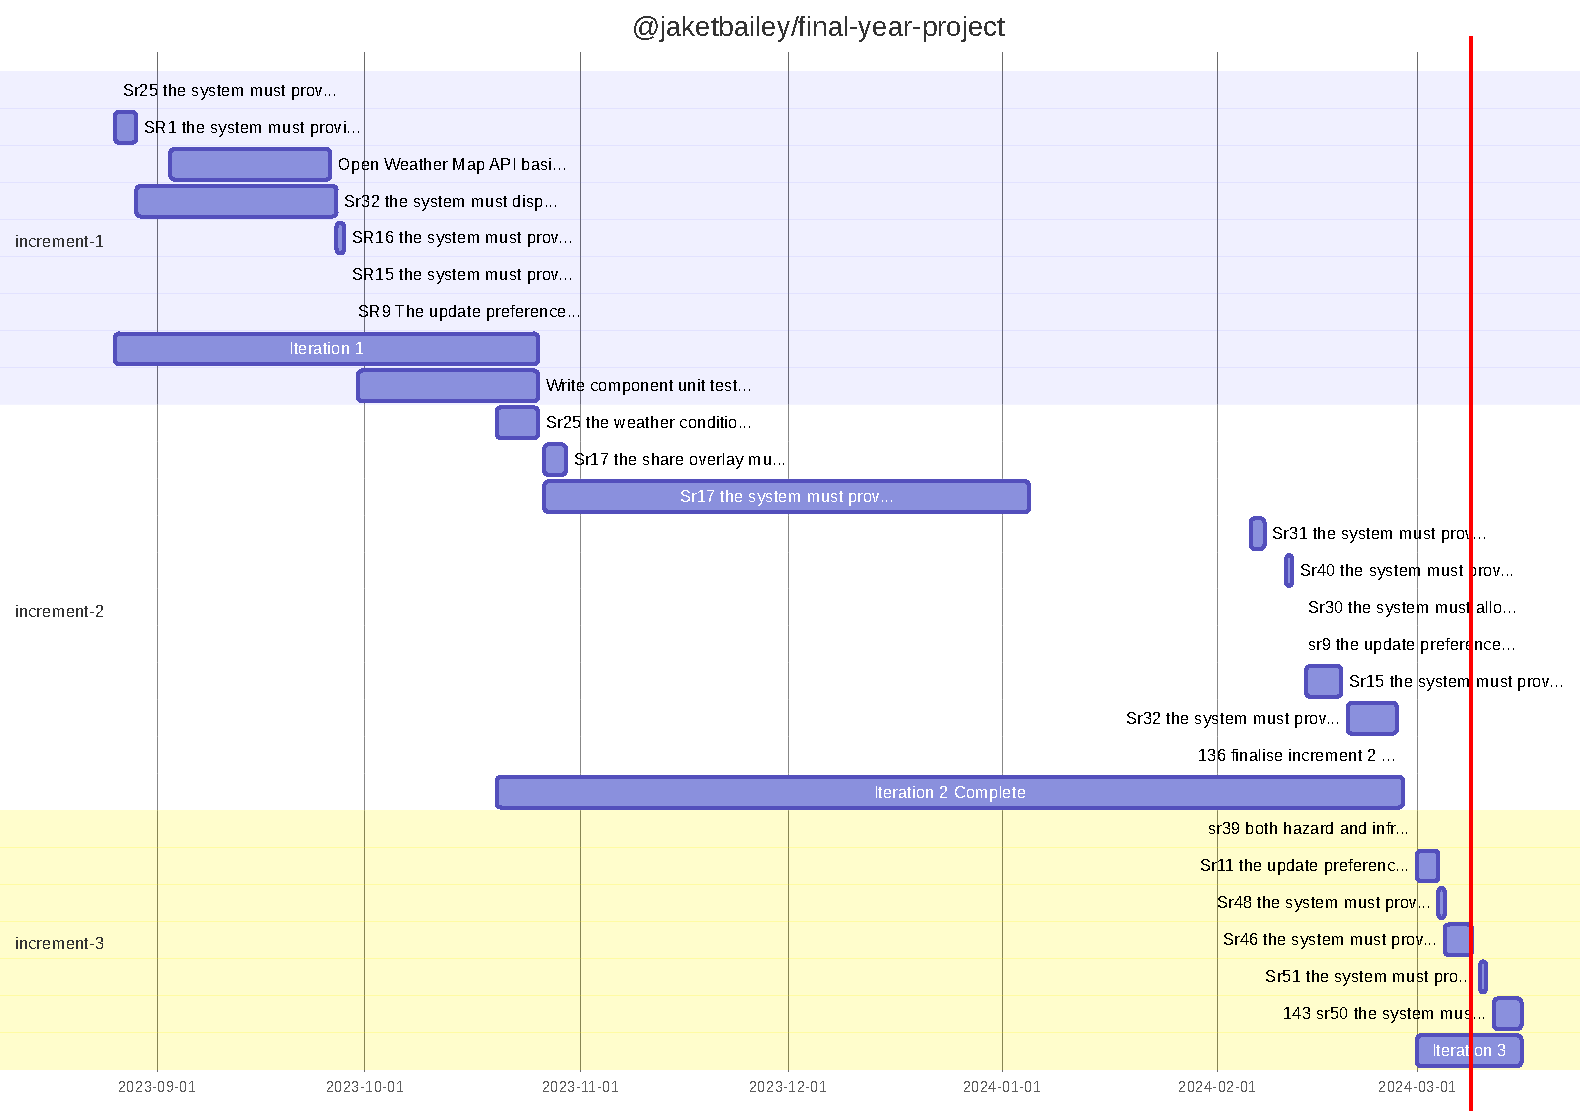
\includegraphics[width=0.9\linewidth]{figures/dev-gantt.pdf}
        \caption{Actual Development Gantt Chart}
        \label{fig:development-gantt}
    \end{figure}
    \newpage
\end{landscape}
\subsection{Project Management}
Overall the project was managed more effectively than originally planned, running ahead of schedule throughout the academic year. The extra time allowed for refinements and improvements without the pressure of an immediate deadline. Constant feedback from the client yielded a more developed understanding of the requirements, the project direction and suggestions for new requirements. The requirements originated as user stories, broken down into smaller, system requirements \see{requirements:user-stories}. Doing so made the use of GitHub projects \see{pm:kanban} and issues more effective with the ability to visualise project progress, further aiding an iterative agile development process \see{methodology:chosen}.

To summarise, the project was managed effectively, except for the early start of iteration 1. The time spent on both development and report writing was well-balanced around other modules and commitments, limiting the chance of burnout. The primary issue was the early stages where development decisions were made without designs and requirements resulting in a knock-on effect in later project stages when integrating more complex features with pre-existing code. It is critical to ensure the project is well planned and development doesn't begin until the requirements and designs are complete to limit the chance of future rework and refactoring.

\clearpage
\section{Evaluating Requirements}
\label{evaluation:requirements}

For this project, assessing its success based solely on the fulfillment of the defined requirements might not provide a comprehensive evaluation. All requirements were established ahead of the three development iterations, with a revision made after primary research was completed \see{fig:research-results}. User stories were created and broken down into smaller system requirements, which were assigned to the development iterations based on priority order via the MoSCoW method \see{chap:requirements}. Further analysis was required to determine if all requirements were met and if they combined to meet all objectives. For all discussion surrounding the project's objectives \see{chap:reflection-and-conclusion}.

\subsection{Unmet Requirements}
Overall, 47 of 51 system requirements were met \see{evaluatedrq}. The four requirements not met were due to the prioritisation of other requirements, the missed requirements were not critical to the system's functionality. They were not met because of the focus on \hyperref[SR:50]{SR50} at the end of development which was a complex but ideal feature to implement. Therefore, some of the initial requirements were not met. Should there have been extra development time, these would be the first to be implemented.

The requirements missed were primarily from 'User Story 05' \see{tab:user-story-05} as these were marked as 'Could' with the MoSCoW method. These focused on integrating weather data into the route planning algorithm. Whilst consideration occurred for extending development and implementation, there was no such weather data API that could serve effectively for this specific purpose. This was due to limited funds and the complexity of the feature.

\subsection{Met Requirements}
\label{evaluation:requirements:met}
All requirements met can be evidenced by the work undertaken within the 'Implementation' chapter of this report \see{chap:implementation}. The routing machine provides users with core routing functionality and customisability (\hyperref[tab:user-story-02]{User Story 02}), whilst providing the user with the ability to export and share routes locally or to external services such as Garmin, Strava and Google Drive (\hyperref[tab:user-story-03]{User Story 03}, \hyperref[tab:user-story-04]{User Story 04}) \see{fig:garmin-connect}. Furthermore, the map component enables users to view and manipulate the route (\hyperref[tab:user-story-06]{User Story 06}) \see{fig:route-import}.

Many requirements were reliant on others to be built first, therefore the MoSCoW method was used to determine the prioritisation based on user feedback with consideration of requirements' dependencies on other requirements. This enabled a functional, well-rounded system to be developed in a logical order, with a focus on modularity. Reflections on the requirements and objectives can be found in the conclusion \see{reflection-and-conclusion:outcomes/objectives-met}.

\begingroup
\setlength{\tabcolsep}{10pt} % Default value: 6pt
\renewcommand{\arraystretch}{1.5} % Default value: 1
\begin{table}[!htb]
\caption{Requirements Evaluation}
\label{evaluatedrq}
\small
    \begin{tabularx}{\textwidth}{ p{1cm} p{11cm} p{1cm} }
        \hline
        ID & Description & Met? \\ 
        \hline
        & \textbf{\hyperref[tab:user-story-01]{User Story 01}} \\
        \hyperref[SR:1]{SR1} & The system must provide a route configuration panel. & Y\\
        \hyperref[SR:2]{SR2} & The route configuration page must provide a starting and destination location input field. & Y\\
        \hyperref[SR:3]{SR3} & The route configuration page must suggest accurate geolocations based on the location inputs.  & Y\\
        \hyperref[SR:4]{SR4} & The route configuration page must determine the geolocation based on the user input. & Y\\
        \hyperref[SR:5]{SR5} & The route configuration page must plan the route once two or more locations are input. & Y\\
        \hline
        & \textbf{\hyperref[tab:user-story-02]{User Story 02}}  \\
        \hyperref[SR:6]{SR6} & The system must provide an overlay window to allow the user to update routing preferences. & Y\\
        \hyperref[SR:7]{SR7} & The update preferences overlay must provide options to 'avoid' along the route. & Y\\
        \hyperref[SR:8]{SR8} & The update preferences overlay should provide a 'via' user input field. & Y\\ 
        \hyperref[SR:9]{SR9} & The update preferences overlay should provide a 'leave time' user input field. & Y\\ 
        \hyperref[SR:10]{SR10} & The update preferences overlay should provide a 'arrive time' user input field. & Y\\ 
        \hyperref[SR:11]{SR11} & The update preferences overlay could provide a 'round trip' user input field. & Y\\ 
        \hline
        & \textbf{\hyperref[tab:user-story-03]{User Story 03}}  \\
        \hyperref[SR:12]{SR12} & The system must provide an option to export the planned route. & Y \\
        \hyperref[SR:13]{SR13} & The system must provide an export feature to export the route to the 'GPX' file format. & Y\\
        \hyperref[SR:14]{SR14} & The system should provide an export feature to export the route to the 'GeoJSON' file format. & Y\\ 
        \hyperref[SR:15]{SR15} & The system must provide an export online (to Google Drive, OneDrive and/or other cloud services) & Y\\
        \hline
    \end{tabularx}
\end{table}
\clearpage

\begin{table}[!htb]
    \ContinuedFloat
    \caption{Requirements Evaluation Continued}
    \label{evaluatedrqextended}
    \small
    \begin{tabularx}{\textwidth}{ p{1cm} p{11cm} p{1cm} }
        \hline
        ID & Description & Met? \\ 
        \hline
        & \textbf{\hyperref[tab:user-story-04]{User Story 04}}  \\
        \hyperref[SR:16]{SR16} & The system should provide a share functionality overlay. & Y \\
        \hyperref[SR:17]{SR17} & The share overlay should provide an option to share direct over email. & Y\\
        \hyperref[SR:18]{SR18} & The system could provide an option to share the route direct to Strava. & Y\\ 
        \hline
        & \textbf{\hyperref[tab:user-story-05]{User Story 05}} \\
        \hyperref[SR:19]{SR19} & The system must provide the user with a weather condition overlay. & Y \\
        \hyperref[SR:20]{SR20} & The weather condition overlay must provide the user with the weather for the current day. & Y\\
        \hyperref[SR:21]{SR21} & The weather condition overlay should provide the user with the weather for the next week. & Y\\
        \hyperref[SR:22]{SR22} & The weather condition overlay could provide the user with the option to enable weather conditions in the route planning algorithm. & N\\ 
        \hyperref[SR:23]{SR23} & The weather condition overlay could provide the user with suggestions on the best days to cycle. & N\\
        \hyperref[SR:24]{SR24} & An option to include weather in route planning could be provided, ensuring the user enters the planned day to ride & N\\ 
        \hline
        & \textbf{\hyperref[tab:user-story-06]{User Story 06}}  \\
        \hyperref[SR:25]{SR25} & The system must provide the user with an interactive map to display the planned route. & Y \\
        \hyperref[SR:26]{SR26} & The interactive map must allow the user to zoom into parts of the planned route. & Y\\
        \hyperref[SR:27]{SR27} & The interactive map should allow the user to select parts of the route and receive detailed information about that subsection of the route. & Y\\
        \hyperref[SR:28]{SR28} & The interactive map should allow the user to select and drag the planned route to modify its path. & Y\\ 
        \hyperref[SR:29]{SR29} & The system should display an elevation graph for the planned route beneath the interactive map. & Y\\
        \hyperref[SR:30]{SR30} & The system must allow the user to measure chosen sections of the route & Y\\
        \hyperref[SR:31]{SR31} & The system must provide multiple map layers to give users the greater options when viewing the route & Y\\ 
        \hline
        & \textbf{\hyperref[tab:user-story-07]{User Story 07}}  \\
        \hyperref[SR:32]{SR32} & The system must provide a user input modal to input Hazard and Infrastructure Data. & Y \\
        \hyperref[SR:33]{SR33} & The hazard input modal must provide a Type drop-down menu based on the OSM Hazard Types. & Y\\
    \end{tabularx}
\end{table}
\clearpage

\begin{table}[!htb]
    \ContinuedFloat
    \caption{Requirements Evaluation Continued}
    \label{evaluatedrqextended2}
    \small
    \begin{tabularx}{\textwidth}{ p{1cm} p{11cm} p{1cm} }
        \hline
        ID & Description & Met? \\ 
        \hline
        & \textbf{\hyperref[tab:user-story-07]{User Story 07 Cont.}}  \\
        \hyperref[SR:34]{SR34} & The hazard input modal should provide a date entry point to specify the date the hazard was seen. & Y\\
        \hyperref[SR:35]{SR35} & The hazard input modal must provide a submit button to add the hazard to the hazard index. & Y\\
        \hyperref[SR:36]{SR36} & The infrastructure input modal must provide a Type drop-down menu with different types of cycling/road infrastructure & Y\\
        \hyperref[SR:37]{SR37} & The infrastructure input modal must provide a date entry point to specify when the bad infrastructure was found & Y\\
        \hyperref[SR:38]{SR38} & The infrastructure input modal should provide an input box providing the user with the option to supply more detail & Y\\
        \hyperref[SR:39]{SR39} & Both Hazard and Infrastructure data should be displayed on the map, with an option to toggle on/off, and report errors & Y\\
        \hline
        & \textbf{\hyperref[tab:user-story-08]{User Story 08}}  \\
        \hyperref[SR:40]{SR40} & The system must provide a map layer to include key waypoints. & Y \\
        \hyperref[SR:41]{SR41} & The waypoint layer must provide locations of accommodation along the route. & Y\\
        \hyperref[SR:42]{SR42} & The waypoint layer should provide locations of tourist points along the route & Y\\
        \hyperref[SR:43]{SR43} & The waypoint layers must be able to be toggled on and off & Y\\
        \hyperref[SR:44]{SR44} & Each waypoint must be clickable to provide extra detail on each point & Y\\
        \hyperref[SR:45]{SR45} & Each waypoint should have a button to add stop along the route and the route will be re-plotted via the waypoint. & Y\\
        \hline
        & \textbf{\hyperref[tab:user-story-09]{User Story 09}}  \\
        \hyperref[SR:46]{SR46} & The system must provide an option within the route planning modal to select the rider type. & Y\\
        \hyperref[SR:47]{SR47} & The system should provide an option within the route planning modal to select the fitness level of the rider. & N\\
        \hline
        & \textbf{\hyperref[tab:user-story-10]{User Story 10}}  \\
        \hyperref[SR:48]{SR48} & The system should provide an import option for GPX files. & Y\\
        \hyperref[SR:49]{SR49} & The system should provide an import option for GeoJSON files. & Y\\
        \hline
        & \textbf{\hyperref[tab:user-story-11]{User Story 11}} \\
        \hyperref[SR:50]{SR50} & The system should provide an export to Garmin Routes. & Y\\
        \hyperref[SR:51]{SR51} & The system should provide an option to share to different social media platforms. & Y\\
        \hline
    \end{tabularx}
\end{table}
\endgroup

\clearpage
\section{Limitations}
\label{evaluation:limitations}

This section will discuss the limitations found during the development of the project. The limitations are based on the requirements and the development process, with a focus on round-trip routing, route imports with LRM, compatibility, and cloud-based route-sharing limitations.

\subsection{Round Trip Routing}
The first limitation found was with the routing algorithm and library used to integrate with Leaflet (Leaflet Routing Machine (LRM) and OpenRouteService (ORS)). The library was not as customisable as initially thought, leading to the need to fork the connecting library between Routing Machine and ORS to enable round-trip routing. LRM requires a minimum of two inputs (A to B), therefore when implementing round-trip, it was not possible to integrate this into the LRM without significant changes to the library. This feature should have proven simple, however, the limitations of LRM required DOM elements in the UI to be hidden to enable the round trip feature, with custom triggers to remove the 2 input minimum. Ideally, LRM would not be used and a custom routing machine would be built from scratch for future versions of the system.

\subsection{Route Import}
Furthermore, another limitation found when integrating LRM was the inability to import routes. Currently the system imports routes by parsing either a GPX or GeoJSON file, taking the route coordinates and adding them as a 'Waypoint' in LRM. Each 'Waypoint' acts as a 'via' position in the route. Consequently, in long routes, there can be hundreds of 'Waypoints' which are all added as 'via' points in the UI. This caused many issues when querying geolocation for each waypoint whereby the API would block access due to the number of requests. To resolve this, the system will not make geolocation requests when there are six or more waypoints. The drawback to this is that the system will not provide named locations for waypoints when there are six or more waypoints. These issues with LRM further highlight the need to build a custom routing machine.

\subsection{Compatibility Issues}
Compatibility is another limitation where the system is currently only compatible with desktop devices, having little responsiveness to support mobile. This is because the focus was on desktop-based route planning rather than mobile, however, in future iterations, mobile support will be considered \see{design:assumptions/decisions}. Minimising the amount of overlays on the UI will also be a core focus to improve the user experience, to integrate the overlays into the core UI elements.

\subsection{Cloud-based Route Sharing}
A final limitation is the lack of a cloud-based server to store user data and routes. This was a feature that was considered, however, due to the complexity and time constraints, it was not feasible to implement. This would have allowed users to save routes and access them from different devices, as well as share routes with other users. These routes would also be implemented into the social sharing functionality. Direct links to routes would be generated and shared, with the ability to view shared routes natively in the system.

\section{Future Work}
\label{evaluation:future}

The four outstanding requirements that were not met will be migrated into iteration 4. The main focus will be integrating weather data within route planning. The following limitations will also be addressed:
\begin{itemize}
    \item Rewriting the routing machine to increase modularity, include round trip and increase code efficiency.
    \item Improving route import, including support for Garmin, Strava and other services.
    \item Mobile support and minimise the number of floating overlays and integrate into core UI elements.
    \item Implementing a cloud-based server to store user data and routes.
\end{itemize}
Addressing the limitations of the project will be the primary focus, however, the following desired improvements will be implemented:
\begin{itemize}
    \item Implementing a system to allow users to save routes and access them from different devices.
    \item Implementing a system to allow sharing of routes with other users.
    \item Implementing native avoid areas in the route planning algorithm.
\end{itemize}

\section{Conclusion}
\label{evaluation:conclusion}

The project was precisely managed, ensuring a balance between development tasks and other project commitments. Through constant effort, the established requirements were largely fulfilled, marking a significant achievement in system development \see{evaluation:requirements:met}. Recognising the project's limitations \see{evaluation:limitations}, proactive measures were taken to address them, accompanied by a clear idea for future work. This culminates in the following chapter which offers a reflective analysis of the project's accomplishments and the goals achieved.



